\section{Background and Related Work}
\label{sec:background}

\subsection{Grounding}
Symbols of a symbolic system such as words in a natural language are typically processed and manipulated in a purely formal manner, without direct reference to their real-world concepts.
The question arises, how these symbols can acquire meaning and be connected to the real world without any external interpreter, in other words how the symbols can be grounded in the real world.
This is known as the symbol grounding problem \citep{Harnad1990}.
Hereby, \citet{Harnad1990} describes that a high-order \emph{symbolic representation} needs to be grounded bottom-up in two non-symbolic representations.
\emph{Iconic representations} refer to analogue representations of sensory input like for instance vision in the retina.
These representations are mapped to \emph{categorical representations} which are filtered clusters of the iconic representation.
These categories are assigned so-called elementary symbols, in which symbolic representation are grounded.

In computational models this problem is tried to be solved in multiple ways.
Recent large language models (LLMs) such as BERT \citep{Devlin2019} or GPT-3 \citep{Brown2020} are often trained on big amounts of text corpora produce impressive results on many tasks in Natural Language Processing.
Meaning of symbols emerges through relating it to its surrounding context of other symbols it appears in.
In this way, their only way of learning, how to generate language as well as solve these tasks is to find patterns of how words and sentences are used in these large corpora.
This approach is however criticized by many researchers, since the meaning of symbols is still not connected to the real world and only relies on other symbols in an infinite recursion.

In \citep{Bender2020}, the authors argue that meaning is bound to a communicative intent.
These are the purposes of why humans are using language.
The intent is always embedded in a broader context that exists outside the language itself.
This context includes the real world, but also the background knowledge of the speaker as well as interlocutors or reason for what the speaker is saying.
By grounding the intent in this context, it becomes meaningful.
Only with this step, the intent can be interpreted by the listeners.
% This intent is connected to the real world that exists outside of language, in other words it is grounded in the world.
% SD: Not just real world, also to background knowledge and what the person wants to do. 
% SD: Grounding is more related to interpretability of expressions rather than intent. Without grounding they cannot be interpreted. The intent shapes WHAT referring expressions are generated in what contexts of the real world.   Hence, intent is a meta thing connecting world, language, knowledge and agent’s experience.
% DK: first part included, referring expressions are included below (done)
This grounding is missing when models only train on abstract textual representations of the world \citep{Regier1996,Landau1998}.

\citet{Bisk2020} argues that a multimodal approach, including for instance perception as well as social context, is needed to learn meaning in a broader context.
One added modality to ground language is often visual input.
Hereby, the model needs to learn how to associate linguistic concepts in text corpora with features, extracted from visual input.
For instance, a model can learn to associate the noun "dog" with an animal seen in an image or associate the action of "jumping over" with the animal being above an object.
\cite{Roy2002} for example studies how an artificial agent can ground spatial relations with a visual scene of geometric shapes.
Hereby, the agent builds up hierarchical knowledge that is used to produce correct description in a rule-based manner.
In more recent research, complete natural language utterances as well as the visual representations are mapped into an embedding space.
By aligning both representations, natural language can be connected to a second modality.
Other research explores how to ground smaller parts of the utterances, as phrases and words and combine them compositional \citep{Larsson2018,Kollar2010}.
This might allow artificial machines to learn grounded concepts more general.

Furthermore, artificial agents can learn to ground language through dialogue, either with human tutors or with other artificial agents.
\citet{Skocaj2011} for example teach a robot different objects and concepts.
By asking questions and participating in the dialogue with a human tutor, the robot builds up and verifies beliefs, and connects them to language and its visual input.
\citet{Lauria2001} follow a similar approach where a robot is taught to follow instructions to generate a map of its physical surroundings.
By incorporating dialogue and deep-level reasoning questions the learning gains are enhanced.
How artificial agents can ground language in dialogue between each other will be studied in this thesis.
Section \ref{sec:background:language-games} gives an insight in the state of the research.


\subsection{Referring expressions}
\label{sec:background:re}
A specific case of grounding linguistic information in visual input are referring expressions.
While a general linguistic expression can be grounded in multiple regions of a visual scene, referring expressions are expected to refer to a unique region \citep{Sanchez2022}.
Given for example a visual scene with multiple pens lying on a table, the word 'pen' can be grounded in all visible objects.
A referring expression like 'the red pen on the left' in contrast would only refer to one specific object.
Referring expressions are however not limited to refer to one single entity, but might also refer to a group of objects as for instance with 'the green pens'.
Still they refer to a specific subset of entities and concepts.

Hereby, \citet{Krahmer2012} classify referring expressions into four categories:
\emph{One-place predicates} refer to one single entity in the visual scene without.
By this, the entity is identifiable without using another entity as basis.
Often, the referring expressions includes intrinsic attributes of an object or absolute locations in the scene as in 'the red pen on the left'.
\emph{Relational} referring expressions refer to entities via other entities in the scene.
Accordingly, a relating between the target entity and distractors is described.
This includes for example spatial relations like 'the pen behind the cup' or relations based on the entities' properties like 'the largest pen'.
Referring expressions can also identify \emph{sets} of entities.
Instead of uniquely referring to on single pen, the referring expression 'the green pens' refers to all objects that are pens and that are green.
Finally, \emph{gradable} referring expressions involve gradable properties as opposed to absolute values.
For example, given the referring expression 'the tall building', 'tall' is a gradable property because it can be measured on a scale.
The success of the referring expression depends on how well it captures the intended level of height compared to other buildings.
By this, vagueness is introduced and referring expressions depend on context, either present in the visual scene or pragmatic context.

One of the main challenges of referring expressions lies in ambiguity.
Ambiguity is introduced in two forms.
First, there is an inherent difference in natural language and the real world it is grounded it, also described in the symbol grounding problem.
The nature of the world is continuous, while natural language being a formal symbol system uses discrete symbols.
In especially, natural language utilizes a very limited set symbols to represent the world.
When trying to map continuous concepts to this limited set of discrete symbols, information nesecarilly gets lost.
Apparent examples are the color systems in human languages.
While color grades exist on an infinite spectrum in the real world, languages combine certain color grades into categories \citep{Zaslavsky2018}.
The word 'red' for example refers to many different shades of red.
Even more, the shades of color it actually refers to depends also on the pragmatic context and the people uttering it \citep{Monroe2017}.
The same also applies to spatial references.
References like 'near to' or 'left to' might refer to objects that are touching each other, but in other contexts also are kilometers away from each other.

The other form of ambiguity is introduced through under-specification of the speakers (e.g. \citet{Dobnik2021}).
When interlocutors interact in a dialogue, they share some common knowledge.
The first interlocutor might presuppose that the second interlocutor knows a certain fact.
Based on this, they might utter a referring expression that together with this shared fact uniquely identifies an entity.
However, the referring expression on its own is under-specified and might refer to multiple entities.
Given for example the following situation:
Two people are in a room with their beverages standing on the table and Person A requests his beverage from Person B.
A referring expression like 'the beverage close to me' would uniquely identify on of the beverages.
Despite that, Person A might more likely use 'the beverage' to refer to theirs.
On its own, the referring expression is under-specified and can refer to both of the present beverages.
However, both persons share the fact that the targeted beverage belongs to person A, which disambiguates the referring expression in this context.
In another context, the shared fact would be that Person A wants to try the beverage of Person B.
Again, this fact would disambiguate the referring expression, but now refer to the second beverage.
The referring expression is the same in both contexts, but refers to two different entities.
This creates a challenge for computational models, that need to understand and generate referring expressions if they are only presented with the text, but not with the shared context.

The research of referring expressions can be split into two fields: referring expression generation (REG) and referring expression comprehension (REC).
In \textbf{referring expression generation}, computational models are trained to generate a referring expression that uniquely identifies an entity given some perceptual, often visual input.
The research goes back into the 70s, where \citet{Winograd1972} developed an algorithm to generate referring expressions step by step, taking into account the context and the information available at each stage of the generation process.
A similar approach is described in \citep{Dale1995}.
Their incremental algorithm is based on the salience of the properties of the present target object and distractor objects.
The most salient properties are considered first, and added to the referring expression until the referring expression is unambiguous.
In other words, the object is described unambiguously using the lowest number of words.

\begin{figure}[ht]
    \centering
    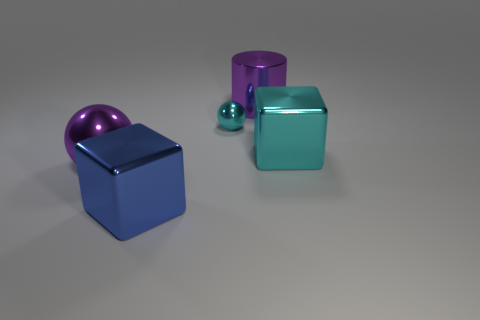
\includegraphics[width=0.5\linewidth]{figures/CLEVR_dale-5.png}
    \caption{The target object in this scene is the \emph{small turquoise sphere}. Using the incremental GRE-algorithm, the target object can be uniquely referred to as \emph{turquoise sphere}}
    \label{fig:incremental-algorithm}
\end{figure}

Given for example the scene in Figure \ref{fig:incremental-algorithm}.
Objects in this scene have three attributes that we consider in the following order of salience: a shape, a color and a size.
This order defines, which attributes can be left out, while still identifying the object uniquely.
The target object in the given scene is the \emph{small turquoise sphere}.
In the first step, the attribute with the highest salience, the shape, is selected from the target object.
This produces the referring expression \emph{sphere}.
In the next step, it is checked if there are also distractors, described by this referring expression.
In our case, both cubes and the cylinder are already disambiguated, but the purple sphere can still be described by the produced referring expression.
Therefore, the algorithm also adds the next lower salient attribute, the color to the referring expression, which produces the \emph{turquoise sphere}.
With this, also the last remaining distractor is as well disambiguated, and the referring expression describes the target object uniquely.
The size, the least salient property is therefore not necessary in the referring expression.
This algorithm will be utilized in this thesis and will be referred to as \emph{the incremental GRE-algorithm}.

Additional to generating an efficient disambiguating referring expressions, a challenge also lies in processing the visual input.
This especially applies to spatial and geometric positions and relations of objects in a scene, where models struggle to extract geometric information from visual features \citep{Kelleher2017}.
More complex scenes also involve multiple perspectives, where the models are tasked to produce referring expressions that depend on the spatial perspective of the speaker and the listener \citep{Ahrens2022,Lee2022}.
In \citep{Dobnik2021}, visual dialogue is analyzed where speakers have different views on cups that are placed on a table.
When speakers refer to a certain cup, they need to take the perspective of the listener to disambiguate the referring expression; for instance in the referring expression 'the cup on the left', \emph{left} is dependent on the speaker's and listeners' spatial position in relation to the cup.

Current research focuses hereby on generating relational referring expressions, which add more complexity to the task \citep{Ghanimifard2017,Ghanimifard2019,Ramisa2015,Liu2023}.
Models need to first extract visual features of multiple objects from the scene.
Of these extracted objects, a meaningful landmark object needs to be found which helps to refer to the target object.
Finally, they need to find proper relations between them to describe the target object.
Relations can be mostly based on the geometric and spatial relation of two objects (e.g. above/below), while the function of objects play a stronger role in other relations (e.g. over/under) \citep{Coventry2005,Dobnik2013}.

% By doing this, the models ground parts of their language in another perception of the real world and get a step closer to learn the actual meaning.
% SD: They learn how to interpret expressions against some representation. Hence, a reference is a relation between a description and some entity, it’s interpretation. Without this connection referring expressions are useless as we do not know how to interpret this. Textual models might be good for general knowledge such as factual information from news and Wikipedia but as soon as we have NLP applications that interact with other domains, e.g. a ticket booking system or a situated robot involved in patient care, we need to connect language to some other representations to make language interpretable.
% DK: done

Referring generation tasks can be hard to evaluate, since often there are many possible referring expressions that are possible and uniquely identify the target object \citep{Mao2016}.
Instead, the task can be turned around: A model needs to identify an object when presented with a referring expression.
This is called \textbf{referring expressions comprehension}.
Many challenges remain similar to the REG task, since the model needs to extract disambiguating visual features from the scenes as well.
However, the goal is typically to select the best matching region of a given choice in a visual scene \citep{Qiao2020}.
They describe seven different approaches how the challenge is approached in the current research.
In \emph{joint embedding} approaches, both visual input and the textual referring expressions are embedded into the same embedding space.
By doing this, the model is able to find similarities and combine them.
In some cases, an attention mechanism is applied on top.
This allows the model to focus on important parts of each representation for the specific task.
\emph{Modular models} are split up in multiple submodels that split up the complete task and solve them step by step.
This helps to reduce the complexity of a task, as well as making more transparent, where models fail and succeed.
\emph{Graph-based models} try to make use of the structure in a visual scene when multiple objects are present and the model is tasked to disambiguate them.
In a first step, the visual features of the image are transferred into a graph that captures objects' properties and their relations.
This graph is then combined with the referring expression to extract, which of the nodes is represented by it.
To give a bigger focus on syntactic and semantic structure in a referring expression (which might get underrepresented by sentence-level representations of e.g. an LSTM), some models utilize \emph{external parsers}.
These make use classical methods as for example dependency parsers, to parse the referring expressions.
\emph{Weakly supervised} models are used when there is a lack of large datasets that annotate the relation between a referring expression and the corresponding regions in the image.
Instead, they can operate on datasets that only include the visual scene with a matching referring expression.
This is done by selecting a matching region in the visual scene and then reproducing the input referring expression from that region.
During testing, the model only extracts the region from a given referring expression.
While most of the described approaches grounding the referring expression in multiple steps, by first identifying possible regions around objects in the visual scene and then combining each proposal with the representation of the referring expression, \emph{one-stage approaches} combine them into one step.
The image is processed as a whole and combined with the embedded referring expression.
The model then predicts a bounding box around the referred entity.
Finally, \emph{Visual-Language pre-training} tries to jointly learn from visual and textual representations, instead of separate visual and textual processors in the other approaches.
Models like ViLBERT \citep{Lu2019} learn joint representations of language and visual input.
These can then be fine-tuned on the specific referring expression comprehension task.

Closely related to the REC task is visual question and answering (VQA) \citep{Ahrens2022,Antol2015,Ilinykh2022,Xu2016}.
In these tasks, a model is given a question about a visual scene.
The goal is to find an answer in the scene and generate an answer.
Central to this is to extract referring expressions from the question and ground them in the visual scene.
In \citep{Johnson2017}, a model is for example shown an image similar to Figure \ref{fig:incremental-algorithm} and asked the question 'Is there a blue cube with the same size as the purple cylinder?'.
To answer this, the model needs to understand two referring expressions and try to ground them in the image.
In some cases the model can't ground a referring expression, when no object in the scene matches the referring expression.
In the paper, it is solved by using a modular design of the model, where in a first step the question is translated into a sequence of instructions that defines, how the model is supposed to extract information from the image.
In the first part, the referring expression is parsed, while in the second part the model grounds it in the visual input.


\subsection{Language Games}
\label{sec:background:language-games}
% \begin{itemize}
%     \item why language games?
%           \begin{itemize}
%               \item origins of language
%               \item flexibility
%               \item efficiency
%           \end{itemize}
%     \item setup of language game
%           \begin{itemize}
%               \item cooperative vs self-interested
%               \item asymetry
%               \item gumbel softmax vs reinforce
%               \item EGG
%               \item bottleneck
%           \end{itemize}
%     \item how does emerged language look?
%           \begin{itemize}
%               \item compositionality
%               \item generalization
%               \item efficiency
%               \item referring expressions
%               \item discriminative vs description
%               \item entropy minimization
%           \end{itemize}
%     \item why relating objects?
% \end{itemize}

In this thesis, referring expression generation and referring expression comprehension are studied at the same time.
This is done by using language games between two artificial agents.
The term 'language games' was first introduced by \citet{Wittgenstein1953}.
Following his argumentation, meaning of words and language is not absolute, but is situated in human dialogue.
Hereby, two interlocutors converse in language games, that define how the utterances are meant and interpreted.
The words' meaning is not just based on the context or surrounding words, but more on the situation, including pragmatic and social context.
The rules in each of these situations differ and therefore the meanings and semantics of words and sentences may differ from situation to situation.
This is summarized as a language game.
These can be any small parts of conversations, for instance between a teacher explaining a new concept to a student, or between two people, discussing a specific topic.
An interjection 'Water!' may be a warning, an answer to a question, a request or something else, depending on the context.
% SD: Because referring expressions are ambiguous participants rely on language games to resolve the reference in context.
% SD: Give an example of a game?
% DK: TODO
This applies as well to the ambiguous referring expressions, as in the example about the beverages described in section \ref{sec:background:re}.
Which referring expression Person A uses to ask for the beverage, depends on the assumed shared knowledge.
With other interlocutors or situations, different referring expressions are uttered.

This reasoning was taken up when trying to train artificial entities to produce a language.
One of the original games is the signaling game, proposed by \citet{Lewis1969}.
These games are composed of a sender and a receiver.
The sender has access to the state of the world, while the receiver does not.
The sender can choose from a fixed set of signals to communicate information to the receiver.
The receiver, upon receiving the signal, must take an action based on that information.
The goal of both sender and receiver is for the receiver to take the correct action in every state, as both players have a common interest in achieving the same outcomes.
Both sender and receiver are rewarded in the same way if the proposed action was correct.
Hence, both agents need to invent a language together, fit to the conditions of the game.

The study of the emergence of an artificial language serves multiple goals.
First, the study of the emergence of artificial language can help to shed light into why and how natural languages evolved \citep{Bartlett2005,Kirby2002,Kirby2008,Noukhovitch2021}.
This approach allows a deep study of the constraints and restrictions that are necessary so that symbols start to be connected with meaning and get grounded in the real world.
Insights in this field might give indications for in which circumstances natural language evolves.
On the other hand, research analyzes how the emerged language looks and how the agents represent information in messages and symbols \citep{Baroni2022,Lazaridou2017,Chaabouni2022,Kottur2017}.
Some studies observe different properties of the emerged languages, such as compositionality, complexity or efficiency, and study how the agents can be biased towards producing a language that holds certain properties.
Eventually, this can produce languages that agents can use in practical applications instead of relying on the predefined unflexible protocols that are currently used.

In language games it is central that the means of communication are very restricted.
Typically, the agents are given a set of arbitrary symbols, a vocabulary, that the agents can use to convey information.
These symbols initially don't have any meaning, but by using and interpreting them repeatedly to solve the task the agents learn to use certain of those symbols, to encode specific information.
By this, a new artificial language emerges between these agents.
The emergence of a language however is highly dependent on the constraints posed on (1) the agents' architectures, (2) the way of communication, (3) the perceptual input for the agents and (4) the task they need to solve \citep{Baroni2022}.

In \citep{Steels2009} two robots are trained by using language games.
The authors explore how spatial language, more specifically language that focuses on spatial positions and movements, emerges when the agents are situated in the real world and can perceive each other.
Two robots equipped with a camera are moving freely in a space until they see each other as well as the target object of the game.
The target object is moved by the researchers, and that movement is registered by both robots.
The robots now need to communicate the movement to each other using language games.
Hereby, the experiments show that when agents are embodied and have a specific view on the surrounding world the capability of aligning their own perspective with the other's is central for the success of communication and the emergence of a language.

In more recent work, deep neural models are utilized for the agents.
Instead of being embodied, agents only receive visual input, without any perception that the other agent is present.
In \citep{Lazaridou2017}, two agents play a discrimination game.
The same set of images is shown to both agents.
While they are unordered for the receiver, the sender always sees the target image as its first image.
The task is now for the sender to communicate the target image in a way that the receiver can discriminate it from the distractors and then point towards it.
Hereby, two of the constraints mentioned above are studied at once.
First, the way of communication is constrained in the way that the sender can only communicate one symbol per message, which results in the agents clustering images into categories that are described with a symbol.
Secondly, two different sender architectures are compared: the 'agnostic' sender that encodes each image separately and then produces the message, and the 'informed' sender that uses convolutions to combine both images for better discrimination.
While both architectures are able to solve the task with an emerged language, the emerged language of the informed sender converges faster and makes use of more symbols than the agnostic sender.

While the previously described examples always study prosocial agents (agents that have a common goal), \citet{Cao2018} examine self-interested agents.
Hereby, multiple agents need to distribute a set of items between them.
Each item has a utility score for each agent that is only visible to themselves.
The goal for each agent is to gain the highest utility score by choosing the correct items.
To do that, the agents first negotiate with arbitrary symbols in a 'linguistic' channel.
At any time, any agent can choose to end the negotiation by proposing how to distribute the items, using predefined symbols in the 'proposal channel'.
These can be accepted or rejected by the other agents.
Their experiments show that in this self-interested setup, the agents utilize the proposal channel well to solve the task, but no language emerges in the linguistic channel.
However, in a similar setup with prosocial agents, they start to utilize the linguistic channel and create an artificial language.
% SD: Examples of architectures from Baroni. The EGG framework.
% DK: TODO

% SD: Give an example of a language games. Symbols are invented at random. However, the constraints of interaction control how new symbols are introduced and when existing symbols are re-used and used. Agents cannot invent unlimited number of symbols to refer to every event the6 encounter as they have limited memory and therefore they are driven by abstraction. On the other hand, the symbols must be flexible enough. The other agent must be able to resolve the symbols they hear based on the context. Hence, a successful interaction is when a describer is producing such symbols that interpreter can easily interpret within the context, here an image. This is also how a reward function is defined and loss is propagated.
% DK: TODO
\subsubsection{Setup of language games}
\label{sec:background:lg:setup}
In this thesis, the language games are studied with prosocial non-embodied agents that are deep neural networks.
They can exchange multiple symbols to communicate after being presented with images.
This is done using the \emph{EGG} framework that allows a high configuration of the agents' architectures, of the ways of communication, and of the technical constraints \citep{Kharitonov2019}.

Using the framework, how the messages of the sender are produced can be controlled.
For instance the sender can send single symbols or use different kinds of RNNs to produce a sequence as a message.
The same applies to the receiver for parsing the message.

Furthermore, a central problem in language games is how to train the sender.
Usually every layer in the receiver model is differentiable and therefore standard backpropagation methods can be used to update the weights in the receiver.
However, the sender's messages are discrete symbols and the loss coming from the receiver can therefore not be simply passed on to the sender.
A classic solution to this problem is to use REINFORCE algorithms \citep{Williams1992} that can handle discrete symbols.
More recently, Gumbel-Softmax relaxation \citep{Jang2017} is used to turn the discrete categorical distribution into a continuous probability distribution.
Doing this, receiver and sender act as a whole deep neural model that can be completely backpropagated with standard methods.
The methods are discussed deeper in section \ref{sec:methodology:optimization}.
When setting up the language game with the EGG, both REINFORCE and Gumbel-Softmax relaxation can be used.

In classical machine learning problems, the models are trained using a train dataset for multiple epochs.
To verify the performance, the model is verified on unseen test samples, which allows to test the ability to generalize its learned knowledge.
Opposed to that, the main goal of language games is not to solve a specific task, but instead the success of communication with a useful emerged language.
Consequently, the agents are trained continuously, and the testing doesn't validate the model on unseen samples, but instead is used to extract the exchanged messages, namely the emerged language.
In other words, during training, the agents are shown randomly drawn samples from the dataset for each game.
This is done repeatedly for $k$ 'games' so that the agents improve and ground their knowledge in the used symbols.
During the testing, the agents are frozen and again randomly drawn samples are shown.
The messages that the agents are exchanging now represent the language that emerged after $k$ language games which can be analyzed.

Section \ref{sec:methodology:egg} explains the framework in more detail.

\subsubsection{Properties of the emerged language}
\label{sec:background:lg:properties}
When agents develop an artificial language, they can learn to use it in different ways.
Several studies research the properties of emerged languages, in particular if they share properties with human languages.
One important property is the capability of forming new meanings by combining multiple symbols in a message, so-called compositionality \citep{Chaabouni2020, Gupta2020,Kharitonov2020, Lazaridou2018}.
\citet{Lazaridou2018} construct a referential game where agents are presented with symbolic input instead of visual input in form of images.
More specifically, each of the objects, target object and distractors, are represented as one-hot vectors where each dimension corresponds to an attribute of the object.
This setup should bias the agents to rely directly on these given attributes in the messages to communicate the target object, instead of first having to extract every possible attribute, for instance  from visual features.
Hence, this helps them to develop a compositional language.
A compositional language should help the agents to communicate objects with unseen combination of attributes during training.
Therefore, to analyze the degree of compositionality in the emerged language, the authors present the agents with new combinations of objects and measure the accuracy.
Even if the accuracy drops lower, the fact that it is still above the random baseline shows that the agents are able to generalize to a certain degree.
Furthermore, they utilize new combinations of symbols in their messages.
However, \citet{Kharitonov2020} show that compositionality is not necessarily tied to the ability to generalize.
In their experiments, non-compositional languages that emerge are able to generalize better than their compositional counterparts.

One essential property of human languages is \emph{Zip's Law of Abbreviation}, in other words that more frequent words tend to be shorter.
In \citep{Chaabouni2019}, the researchers analyze if this law also applies to emerged languages.
They find that without any pressure to produce shorter strings the agents produce a language that follows the inverse rule: the most frequent inputs are associated with longer messages.
Only when long messages are penalized, a language which follows similar rules as human languages emerges.

Finally, a strong focus in the study of emerged languages lies in interpretability \citep{Dessi2021,Lazaridou2017,Chaabouni2021}.
While the agents ground the symbols in their input and certain symbols correspond to certain categories, they do not necessarily align with human categories and words.
However, agents can be biased to use similar categories, as shown in \citep{Lazaridou2017}.
This is done by infusing human labels during training so that the agents ground the visual input not only in their artificial language, but also in human language.
More specifically, their experimental setup is a referential game, where the sender needs to describe the target image in a set of distractors to the receiver.
Alternating with describing the target image to the receiver, the sender is trained to classify its input with human labels.
The results show that this setup doesn't have any negative effect on the communicative success, but instead it only biases the agents to align their vocabulary with human descriptions.
This makes the emerged language much easier to interpret for humans.

\subsection{Artificial dataset}
Language is heavily influenced by the perception and the environment \citep{Hofstadter2013,Dobnik2017,Ji2022}.
This is for instance very apparent in color naming systems across different languages \citep{Zaslavsky2018}.
Which and how many words are used to refer to a specific color is dependent on the perceptual and social context around the speakers.
Different studies show that while all languages tend to share similar basic color categories, some languages' systems are based on different underlying principles.
Color names in the language of the Berinmo people from Papua New Guinea for example  reference natural objects and hence color categories are different from non-referential English color names \citep{Davidoff2001,Steels2005}.
Further, this fact can be applied to more abstract constructs like metaphors, which often reference perceived events in the world \citep{Lakoff1980}.
Perceiving that cats always land on the ground on their feet is for example the origin of the metaphor 'as nimble as a cat'.

This influence on the language by the perception of the world is not only limited to human language learning and evolution, but it as well applies to machines that are trained to produce language.
Many models in different disciplines of Natural Language Processing are trained on datasets such as the MS COCO dataset \citep{Lin2014} or the Flickr30k dataset \citep{Young2014}, which are sourced from uploaded photos in social networks.
While these datasets often contain a large amount of samples, they can contain structural biases.
The photos usually feature and center on specific objects, people or animals.
This is not necessarily a faithful representation of human perception of the world, in which these entities are for instance partially hidden, shown from the back or appear at the edges of the field of view.
The datasets might therefore give a euphemized view on the world.
Furthermore, the datasets can contain underlying patterns in the semantic information of the photos \citep{Hendricks2018,Johnson2017a,Hudson2019}.
For instance, when dogs are photographed, they usually appear running on a meadow.
An image captioning model might learn to predict the caption 'a dog running on a meadow' for all images containing a dog, independently if the dog is actually running on a meadow or sitting in the living room, just because of the higher frequency in the dataset.
In other words, the model might utilize these underlying structural biases rather than relying on the extracted visual information from the image.

Different approaches are taken to mitigate this problem.
While some research focuses on improving the models (e.g. \citet{Hendricks2018,Lu2017}), others create artificial datasets.
Using artificial datasets, one can control exactly which structural patterns occur.
Furthermore, all ground truths as for example spatial positions of objects are known and can be used for training models.
Figure \ref{fig:artificial-datasets} shows several examples of different artificial datasets.
Real world photos often contain a lot of distracting visual information that poses challenges for models to identify the relevant information.
In \citep{Ghanimifard2017} and \citep{Ji2022}, the authors for example create abstract visual scenes that only contain specific concepts, like for instance spatial positions.
With no distracting concepts present, researchers can focus only on the effects of the concept that is relevant for the respective study.
Other datasets consist for example of comic-like scenes \citep{Zitnick2013,Zhang2016}.
These scenes, while still being abstract also contain functional objects.
This adds more complexity for predicting spatial relations.
More recently, datasets are created using 3D environments \citep{Johnson2017a,Lee2022,Ahrens2022}.
Scenes created in this way resemble photos taken in the real world and models can more easily transfer the learned knowledge to real world photos.
Extending this reasoning, several datasets include embodied perspectives.
Images are for example taken from the perspective of a person in the scene \citep{Dobnik2015} or from the perspective of an embodied robot navigating a 3D environment \citep{Hill2021}.

\begin{figure}[ht]
    \centering
    \subfigure[Abstract spatial templates \citep{Ghanimifard2017}]{
        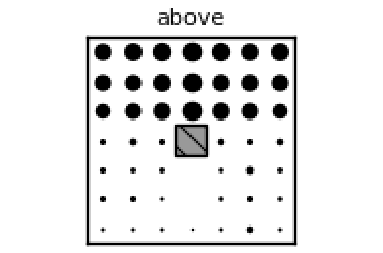
\includegraphics[width=0.3\linewidth]{figures/dataset_Ghanimifard.png}
    }
    \subfigure[Abstract tangram shapes \citep{Ji2022}]{
        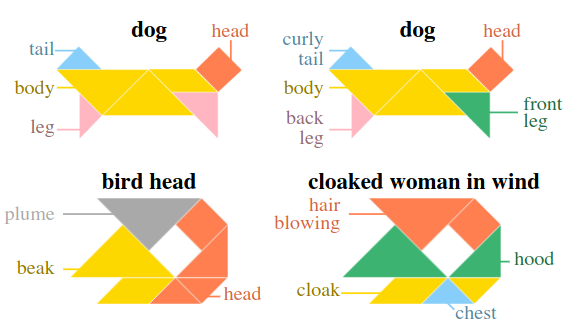
\includegraphics[width=0.3\linewidth]{figures/dataset_Ji.png}
    }
    \subfigure[comic-like scenes \citep{Zhang2016}]{
        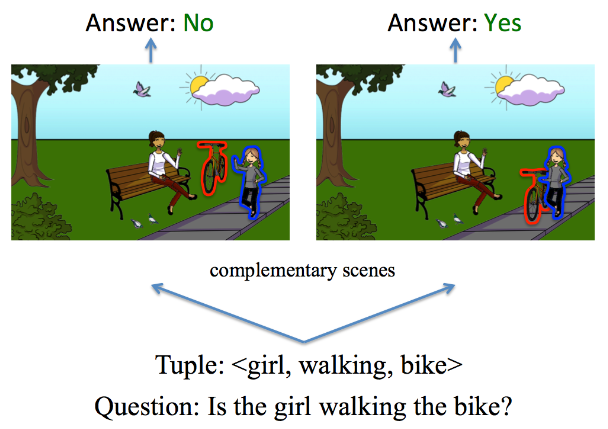
\includegraphics[width=0.3\linewidth]{figures/dataset_Zhang.png}
    }
    \subfigure[3D-generated scenes \citep{Lee2022}]{
        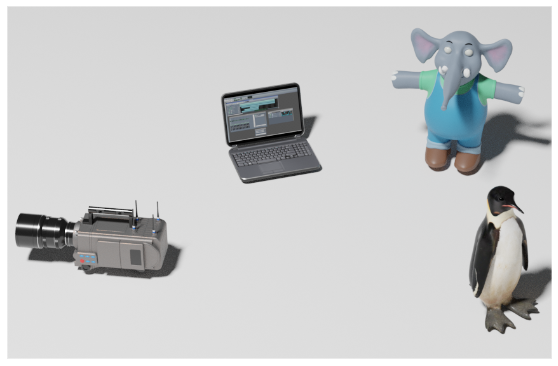
\includegraphics[width=0.3\linewidth]{figures/dataset_Lee.png}
    }
    \subfigure[3D-generated scenes including perspective \citep{Dobnik2015}]{
        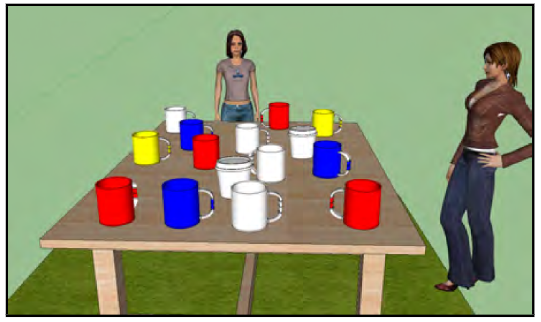
\includegraphics[width=0.3\linewidth]{figures/dataset_Dobnik.png}
    }
    \subfigure[embodied robot in a 3D environment \citep{Hill2021}]{
        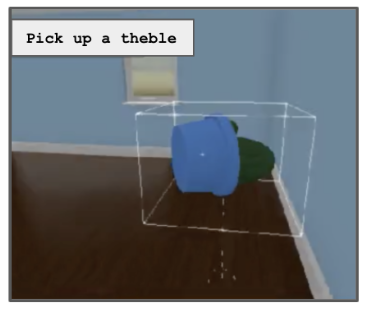
\includegraphics[width=0.3\linewidth]{figures/dataset_Hill.png}
    }
    \caption{Example images from different artificial datasets}
    \label{fig:artificial-datasets}
\end{figure}

This thesis utilizes an artificial dataset for two reasons.
First, all ground truth information about the scenes can be extracted during their generation.
This includes spatial positions of entities placed in the scene, their properties and relations to other entities.
Having all information present, several different tasks for the models can be created using the same generated images.
More importantly, the usage of an artificial dataset allows for perfect control over the bias present in the images, in particular which entities are present, and which properties and attributes they have.
As detailed before, perceptual input shapes the language that describes and interacts with it.
When agents in a language game describe and refer to entities present in a scene, the emerged language is expected to utilize these biases by making use of the controlled attributes in the scenes.
